\chapter{Column-aware方案与缺点}
\label{chp:simple-solution}

\par 在本章中我们会讨论一个容易想到的直接的方案,取名Column-aware方案,此方案没有考虑工程实现的难度,仅考虑我们的目标。然后本章会讨论我们的现有条件,分析这个方案存在的缺点,不能在实际中应用的原因,为我们的第~\ref{chp:cw-cache}章提出的CW-Cache方案提供参考。

\section{Column-aware方案}

\par 由第~\ref{chp:motivation}章我们知道,设计方案需要考虑如何决定复制多少热门的列,以及列的“捆绑”(bundle)放置问题。那么,根据之前的分析,直观上来说,想要基于列的访问热度对集群缓存系统进行列级别的负载均衡,我们的系统需要获得SQL查询任务具体访问的列,才方便对列的热度进行统计,并且根据此热度信息对热门的列进行复制。应用访问数据表的列的信息是由上层计算框架(如Spark SQL)掌握,而alluxio是不知道的,需要计算框架提供给它,拿到这些信息之后,alluxio进行统计,计算列的访问热度,根据热度,计算列需要拷贝的副本数,访问到来时,alluxio根据一定的策略,返回副本中的一个(如果被复制)或者是原表。

% \subsection{简单方案设计}

\par 图~\ref{fig:sim-archi}所示即为本章描述的Column-aware方案的架构的设计。该架构主要有三大组件,最上层计算框架为Spark SQL~\cite{spark-sql}(也可以更换为其他的),中间是基于alluxio\cite{alluxio}实现的列级别的负载均衡系统CW-Cache,底层是分布式文件系统HDFS(Hadoop File System)\cite{hdfs}。

\begin{figure}[]
	\centering
	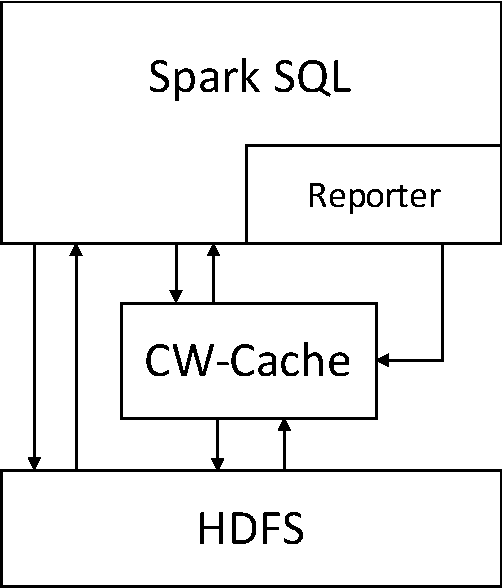
\includegraphics[width=0.4\textwidth]{img/simple-solution/sim-archi}
	
	\caption{简单方案的架构设计。}
	\label{fig:sim-archi}
	%\vspace{-.1in}
\end{figure}

\par 这个列级别的集群缓存系统负载均衡方案工作流程大致如下:当用户给Spark SQL提交一个查询任务,经过一系列转换后,Spark SQL得到具体要访问的列的信息,Reporter负责将这些信息传递给CW-Cache,CW-Cache记录下这些信息,并且将对应列的访问计数器加1。在经过一段时间后,CW-Cache对于缓存的数据表的各个列,均维持有计数器,从中获得各个列的热度(访问频率),然后它根据一定的算法计算出哪些列需要进行复制,复制多少份,哪些列需要“捆绑”在一起放置。当查询任务再此到来,CW-Cache得到应用访问的列,CW-Cache根据一定的策略,在缓存副本(如果有)或者原表中选择相应的列的信息返回给应用,尽可能使得负载比较分散,并且尽力避免出现shuffle,同时更新相关列的访问计数器。以上步骤重复进行。

\par 这个系统是根据我们的目标的很直接简单的一种思路,但是它是不实用的,这样的设计不够通用,比如图~\ref{fig:sim-archi}是针对Spark SQL进行了修改的,如果更换SQL引擎又需要重新实现;其次,这样的设计需要对上层计算层和中间层同时做修改,增加了二者的耦合度,不利于软件开发与维护。下面我们会分析现有条件Parquet和alluxio来解释以上原因。

\section{现有条件}

\subsection{Parquet文件格式}

\par 列式存储有多种格式,Parquet是其中一种被广泛使用的,我们的方案针对Parquet实现,所以这里具体讨论一下Parquet格式。

\par Parquet文件是以二进制方式存储的,因此是不能够直接读取的,Parquet中包括该文件的元数据和数据,所以Parquet格式的文件是自解析的。在Hadoop File System文件系统和Parquet文件中有以下几个概念。

\begin{itemize}
    \item HDFS文件(File):一个HDFS的文件包括数据和元数据,数据分散地存储在多个HDFS块(Block)中。

    \item HDFS块(Block):它是HDFS上的最小的副本(replica)单位,HDFS会把一个Block存储成本地的一个文件,并且维护分散在不同的机器上的多个副本,Block的大小可以根据需求由用户自己配置,Hadoop早期版本默认一个Block大小是128M,Hadoop 2.7.3以及之后的版本默认一个Block的大小为128M。
    
    \item 行组(Row Group):按照行将数据从物理上划分为多个单元,每一个行组包含一定的行数,在一个HDFS文件中至少存储一个行组,Parquet读写的时候会将整个行组缓存在内存中,所以每一个行组的大小是由内存大的小决定的,例如记录占用空间比较小的Schema可以在每一个行组中存储更多的行。

    \item 列块(Column Chunk):在一个行组中每一列保存在一个列块中,行组中的所有列连续的存储在这个行组文件中。一个列块中的值都是相同类型的,不同的列块可能使用不同的算法进行压缩。

    \item 页(Page):每一个列块划分为多个页,一个页是最小的编码的单位,在同一个列块的不同页可能使用不同的编码方式。
\end{itemize}

\par 一般情况下,在存储Parquet数据的时候会按照块(Block)大小设置行组的大小,由于一般情况下每一个Mapper任务处理数据的最小单位是一个Block,这样可以把每一个行组由一个Mapper任务处理,提高任务执行并行度。Parquet文件的格式如下图~\ref{fig:parquet-file-layout}所示。


\begin{figure}[]
	\centering
	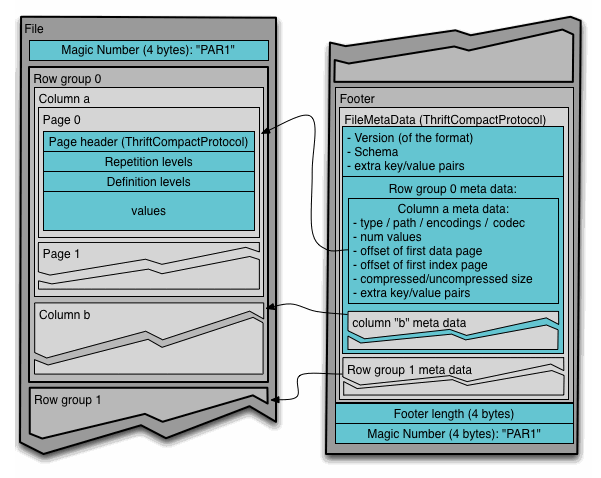
\includegraphics[width=0.5\textwidth]{img/simple-solution/FileLayout}
	
	\caption{Parquet文件格式。}
	\label{fig:parquet-file-layout}
	%\vspace{-.1in}
\end{figure}

\subsection{Alluxio}
\label{subsec:alluxio}

\par Alluxio原名Tachyon,是一个基于内存的分布式文件系统,它是架构在底层分布式文件系统(如Amazon S3、Apache HDFS等)和上层分布式计算框架之间的一个中间件(如Spark、MapReduce、Hbase、Flink等),主要职责是以文件形式在内存或其它存储设施中提供数据的存取服务。在Alluxio出现以前,这些上层的分布式框架,往往都是直接从底层的分布式文件系统中读写数据,效率比较低,性能消耗比较大,而将Alluxio部署在二者之间,以文件的形式在内存中对外提供读写访问服务的话,那么Alluxio可以为那些大数据应用提供一个数量级的加速,而且它只要提供通用的数据访问接口,就能很方便的切换底层分布式文件系统。

\begin{figure}[]
	\centering
	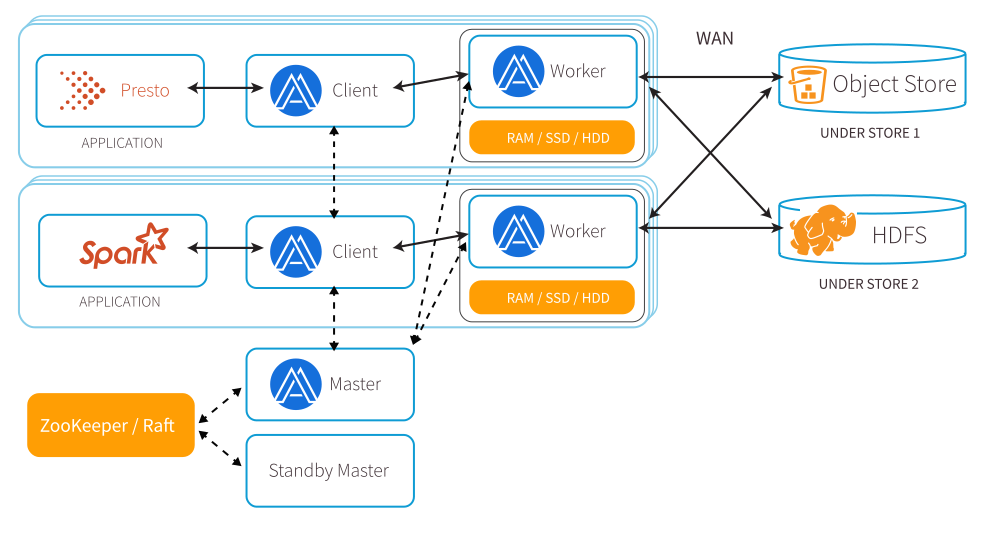
\includegraphics[width=0.8\textwidth]{img/simple-solution/alluxio-archi}
	
	\caption{Alluxio架构。}
	\label{fig:alluxio-archi}
	%\vspace{-.1in}
\end{figure}

\par Alluxio的架构如图~\ref{fig:alluxio-archi}所示。整体框架为主从结构,与Hadoop\cite{hdfs}等类似。主节点为Master,负责管理全局的文件系统元数据,比如文件系统树等;从节点为Worker,负责管理本节点数据存储服务;Client用于Alluxio与用户应用的交互,为用户提供统一的文件存取服务接口。

\par 应用程序访问Alluxio,先通过Client客户端与主节点Master通讯,获取对应文件的元数据,得到存储应用需要的文件的worker,再和对应Worker节点通讯,进行文件存取操作。所有的Worker会周期性地发送心跳给Master,维护文件系统元数据信息,确保自己被Master感知而仍然能在集群中正常提供服务。Master不会主动发起与其他组件的通信,它只是以回复请求的方式与其他组件进行通信。这与HDFS、HBase等分布式系统设计模式是一致的。

\subsection{分析}
\label{subsec:simp-analysis}

\par 从上文的分析可以看出,Parquet文件格式在存储数据表时,先将数据表按行进行“切割”出一个个行组(Row Group),行组内部再按列分成列块(Column Chunk),文件系统里物理存在的文件含有若干行组,同一列的数据物理上并没有存储在一起,并且不同的块(Block)有可能放置在不同的机器上。按照我们在本章提出的简单方案,CW-Cache能够获得Parquet文件的语义信息,希望把热门的列单独提取出来,但是Parquet文件的文件格式决定了这个目标的实现不太容易。直观上来说,需要读取Parquet文件的元数据,找出需要复制的列所在的Block,读取之后将它们拼装成一个新的文件,进行复制,这个过程的产生不可忽略的计算开销和网络通信开销,可能对系统性能造成比较大的影响,抵消负载均衡获得的性能提升。

\par Spark SQL能解析基本的SQL语句并在分布式环境下高效执行,当Spark SQL解析出查询任务需要访问的列,具体的读取任务是交由Parquet文件格式的实现parquet-mr\cite{parquet-mr}来完成的,parquet-mr会读取Parquet文件的footer获取文件的元数据,定位需要读取的列所在的文件块(block)、偏移(Offset)和读取的长度(Length)。然后它把这些信息传递给alluxio,alluxio将结果返回给parquet-mr,parquet-mr将数据解压缩(如果进行了压缩)、拼装之后交给应用进行处理,单独看这个过程,alluxio拿到的信息是一个个“文件片段”,它们甚至不是完成的列块(column chunk),可能只是其中的一小部分,甚至是一个个字节。本章简单方案需要alluxio知道应用读取Parquet文件时的语义信息,而alluxio本身的架构决定了它并不支持这一点,很难将这些零碎的“文件片段”与Parquet存储的数据表的各个列建立关联。如果想要向alluxio传递文件的上下文信息,我们需要额外修改Spark SQL或者parquet-mr的相关模块,增加了上层计算框架和中间层的耦合度,同时因为只在Spark SQL或者parquet-mr进行修改,那么方案仅仅适配Sparrk SQL计算框架或者Parquet这种文件格式,没有通用性,是不好的软件设计。

\par 此外,列的“捆绑”放置(bundling)也是非常困难的。根据~\ref{sec:data-shuffle}和~\ref{sec:shuffle-impact}节,将数据表按照列的粒度缓存并且分开放置会在查询任务中产生表内部的shuffle,且shuffle带来的网络通信开销会对查询任务的执行时间带来不可忽视的影响。~\ref{sec:col-access}节的实验结果表明在列的热度存在差异的基础上,不同热度的列相互之间被共同访问的概率也不一样。于是我们想到可以借助“捆绑”放置(bundling)来减少甚至避免同一张数据表内的数据shuffle。然而这个问题是难以解决的:首先如何得到列的共同访问的模式是困难的。如果一张数据表有$N$列,那么列的共同访问的模式理论上有$2^N$种,在生产环境中是没有足够的资源来同时满足这么多共同访问模式。其次,从系统上来说,alluxio作为通用的内存分布式文件系统,需要为多用户提供服务,只要用户通过alluxio的接口存取文件,alluxio便执行相应的操作,将结果返回即可。alluxio并不知晓每一次的请求来自哪个客户端(Client),它不会维护状态,区分不同客户端的请求。换句话说,不做修改的情况下,alluxio无法得知哪些读访问请求来自同一个客户端的同一个查询任务,那么列的“捆绑”(bundling)放置也就无从谈起。而如果要使得alluxio维护状态信息,首先需要客户端发送请求时附带自己的身份信息,同时alluxio的master需要记录并且进行匹配,大大增加系统的网络、存储、计算开销。

\subsection{总结}

\par 本章主要讨论了一个基于我们的列级别的负载均衡的集群缓存系统的目标而提出的简单直接的方案,它需要上层计算框架将访问的列的信息发给中间层,中间层用以统计各个列的访问热度并且按照一定的策略复制,在请求到来时选择合适的副本传给应用。这个方案有三点缺陷。

\begin{enumerate}
    \item 因为Parquet文件格式是先按照行进行划分,然后再按列进行存储,如果要按照需求把某一列单独抽取出来进行复制,需要读取文件元数据、读取存储该列的各个Block,然后拼装成新的Parrquet文件存放到其他机器,这一系列的操作开销较大;
    \item Spark SQL读取Parquet文件时,调用parquet-mr,传给alluxio的信息仅有所需的文件URI(统一资源标识符)、偏移量和读取长度,并未包含文件的语义信息。想要传递文件上下文信息需要额外对Spark SQL或者Parquet-mr做修改,增加了软件之间的耦合度;
    \item Alluxio作为通用的内存文件系统,为多用户服务,不保存状态信息,不去识别请求来自哪个Client,这意味着alluxio难以知晓哪些列的访问是来自于同一个Client的同一个查询任务,不便于对这些列的缓存作“捆绑”放置(bundle)。如果访问文件时增加Client的身份标识,会大大增加通信开销,同时增加Master维持状态信息的存储、计算开销。
\end{enumerate}

\par 综上所述,本章描述的这个简单方案不具备实用条件,并且难以实现,但对于其缺陷的分析有助于我们更加深刻的理解问题,在现有条件的基础上调整系统设计的方向。在第~\ref{chp:cw-cache}章中我们会介绍实际CW-Cache的系统设计与分析。